\section{Poisson problem}
This section includes several algorithms/kernels, results and analysis of those performances. 
The performance of the kernel setups will be compared and they have been evaluated for $N = 2048$ and \texttt{max\_iter} = $1000$. The chosen parameters gives the refrence algorithm a runtime of $\approx1.5$ secound.

\noindent The main purpose of this section is to find the speedup for difference GPU implementations in reference of the best OpenMP (\texttt{jac\_cpu}) version from previous assignment. The environment variable which determines the wait policy of the threads has not been set to \texttt{OMP\_WAIT\_POLICY=active} is in the previous assignment. The OpenMP is evaluated with \texttt{OMP\_NUM\_THREADS=12}.
The achieved speedups are presented in table \ref{tab:speedup_pos}.

\noindent It has been chosen to validate the implementation of the difference GPU kernels by visualizing their estimates of $u(x,y)$ after the last iteration. This give a visual verfication of the kernel and source implementations. See plots in figure \ref{fig:apped_vis_pos} in the appendix.

\noindent The iterative process is controlled by the host and it uses \texttt{cudaDeviceSynchronize()} to make sure the work of the threads on the devices is done before incrementing the iteration. The iterative process \texttt{while(k < max\_iter)} which includes pointer switchs and new kernel calls is identical for all three GPU versions. Although the kernels are called by different 
kernel launch parameters: \texttt{<<<grid,block>>>}.

\noindent The initialization of the boundary conditions in $u$ and $u\_old$, and of the heating source given by $f$ are done on the on the host. The and copied to the device by using the approiate cuda calls.  
The I/O duration for transferring the initial matrices to the device and the duration of the transferring the estimate of $u$ back to host is included in the total compute time in order to make a fair comparison to the \texttt{jac\_cpu} function.



\subsection{Sequential GPU Jacobi}
The kernel used in the Sequential Poisson is provided in algorithm \ref{alg:jac_v1}. 

\noindent \texttt{jac\_gpu1} is called by the following launch parameters \texttt{<<<1,1>>>jac\_gpu1}. This ensures it only enables one block with one thread. See algo. \ref{alg:app_jac_v1} for the complete source code.

\lstinputlisting[label={alg:jac_v1},caption={Algo. \texttt{jac\_gpu1}.},style=CStyle, linerange={23-33}]{code_3/jac_gpu1.cu}.

\subsection{Naive GPU Jacobi}
The Naive Poisson kernel have been implemented by using one thread per grid point which enables the high parallelism of the device. The implementation uses global memory and line 2-3 shows how the upadted element is determined. The kernel is presented in algo. \ref{alg:jac_v2}.

\lstinputlisting[label={alg:jac_v2},caption={Algo. \texttt{jac\_gpu2}.},style=CStyle, linerange={24-31}]{code_3/jac_gpu2.cu}. 


\noindent The kernel is called by following launch paramters: \texttt{<<<dim\_grid,dim\_block>>>jac\_gpu2} which creates a 2D thread blocks. The 2D grid and block size are given by:
\begin{align}
dim3 \quad &dim\_grid \left(  \frac { N+bs-1 }{ bs },\frac { N+bs-1 }{ bs } \right)  \\
dim3\quad  &dim\_block\left(bs, bs \right)
\end{align}
where $bs=16$ is the number of threads in each block.


\subsubsection{\texttt{nvvp}}
The \texttt{nvvp} analyzing tool tells that the \texttt{jac\_gpu2()} has a "Low Compute Utilization" $\approx 16\%$, presented in figure \ref{fig:computebound}. This is as expected, as all memory is fetched globally in the implementation, and as only few floating point operations are performed every time memory is retrieved. Due to this difficulty, the Jacobi method is memory bound. This could be optimized by splitting up the copying, such that the algorithm could copy and compute simultaneously and hereby reduce the computation time. By using more specialized analysis tools within \texttt{nvvp}, a bandwidth limitation is proposed. This limits also supports the claim that the problem is memory bound.  The solution to the Poisson problem using this algorithm is presented in \ref{fig:jac_gpu2} in the appendix.\\

\begin{figure}[H]
\centering
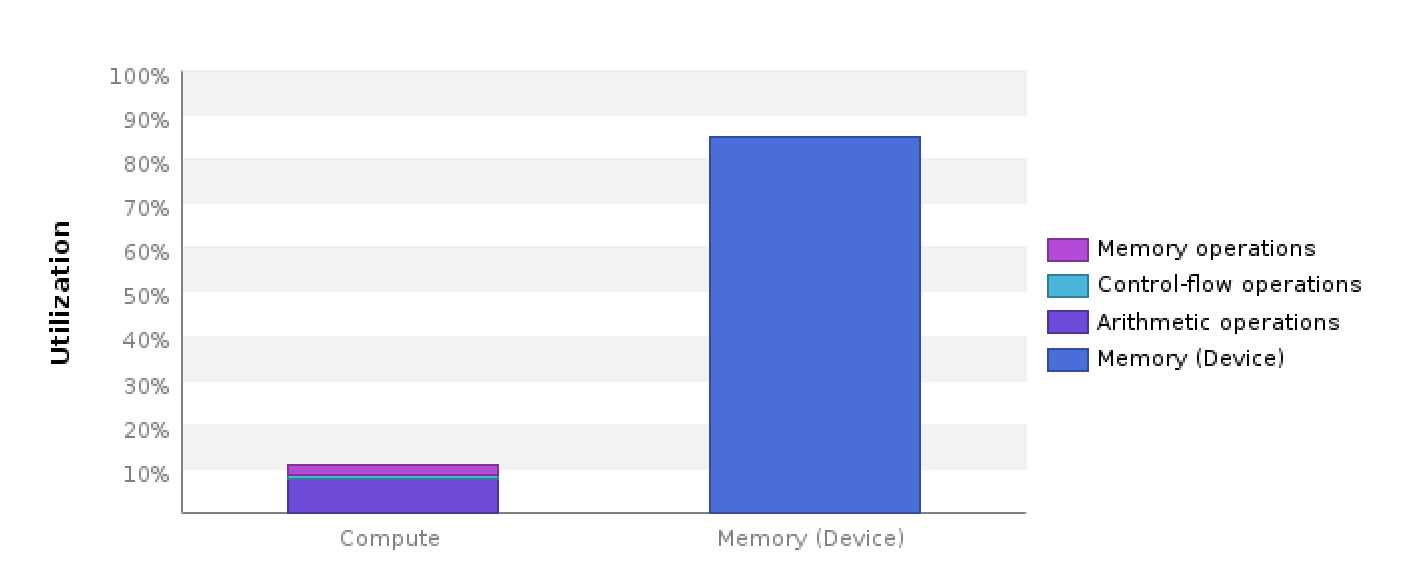
\includegraphics[width=1\textwidth]{data_3/pos_sceenshots/computebound.png}
\caption{The \texttt{nvvp} analysis of \texttt{jac\_gpu2()}. This reports that the algorithm is memory bound as the percentage of utilized memory is much bigger than the utilization of the computation.}
\label{fig:computebound}
\end{figure}

%Vi bruger lang tid på at copiere data, dette kunne blive forbredet hvis man kun kopierede lidt over af gangen . low compute utilization (16\%) pga lang tid om at kopiere. N = 2048, 1000 iterationer. low kernel concurrency.  



\subsection{Multiple GPU Jacobi}
The third version the Jacobi version use multiply (two) GPUs. The problem is hereby split equally between the devices. It has been chosen to create a horizontal split.

\noindent The kernels, \texttt{jac\_gpu3}, used to solve the Poisson problem is presented in algorithm \ref{alg:jac_v3_alg}. 

\noindent The \texttt{cudaDeviceEnablePeerAccess()} method is used to solve the boarder issues between the top and bottom problem as the Jacobi iteration uses the adjacent grid points when updating an element. See the complete source implementation, algo. \ref{alg:app_jac_v3} in the appendix.

\lstinputlisting[label={alg:jac_v3_alg},caption={Algo. \texttt{jac\_gpu3}.},style=CStyle, linerange={26-46}]{code_3/jac_gpu3.cu}

\noindent The kernel is, as in \texttt{jac\_gpu2}, called by the following launch paramters: \texttt{<<<dim\_grid,dim\_block>>> jac\_gpu3}. Noticeable the grid is $N/2$ in the second axis in order to support the dimensions of the each subproblem. The 2D grid and block size are given by:
\begin{align}
dim3 \quad &dim\_grid \left(  \frac { N+bs-1 }{ bs },\frac { N/2+bs-1 }{ bs } \right)  \\
dim3\quad  &dim\_block\left(bs, bs \right)
\end{align}



\subsection{Speedup}
The expected compute speedup is 8x\footnote{PerformanceTuningIntro.pdf, slide 20.} when deploying the algorithm on the GPU compared to the CPU.
Table \ref{tab:speedup_pos} reports the achieved speedups for the three implementations.

\begin{table}[!th]
\centering
\begin{tabular}{l|r}
Algo. & Speedup \\\hline
\texttt{cpu}&1.0000x \\
\texttt{gpu1}&0.0021x \\
\texttt{gpu2}&10.3818x \\
\texttt{gpu3}&16.5419x \\

\end{tabular}
\caption{This table present the speed-ups of \texttt{jac\_gpu1}, \texttt{jac\_gpu2} and, \texttt{jac\_gpu3} in reference to the fastest CPU version from assignment 2, \texttt{cpu()} }
\label{tab:speedup_pos}
\end{table}

\noindent As expected the \texttt{jac\_gpu1} does not gain any improvements. The reason why is the lack of parallelism. Hence there is only launched one block with one kernel.

\noindent The speedup gained by \texttt{jac\_gpu2} is $\approx 10x$ which slightly higher than the expected compute speedup. This can be caused by a version of the OpenMP implementation, which is not fully optimized. If the implementation is sub-optimal the comparison is not fair to the fully parallel implementation on the GPU.

\noindent When splitting the problem into two subproblems the expected speedup is \underline{not} $2x$ between \texttt{jac\_gpu2} and \texttt{jac\_gpu3}. The reason is due to the nature of the Jacobi algorithm. There needs to be shared global memory access between the two devices in order to update the "middle" horizontal boarders elements. The shared global memory, accessed by peer access, is transferred on the PCIe express bus which introduce a latency and therefore not able to scale $2x$. 

% \begin{figure}[H]
% \centering
% \begin{tikzpicture}[scale = 1]
% \begin{axis}[
%     width=10cm, height=8cm,     % size of the image
%     ybar,
%     %symbolic x coords={},
%     xticklabels={\texttt{jac\_cpu},\texttt{jac\_gpu1},\texttt{jac\_gpu2},\texttt{jac\_gpu3}},
%     xtick=data,
%     ytick={0,1,2,9,10,11,15,16,17},
%     ylabel=x,
%     %xlabel=Algo,
%     ]
    
% \addplot table [x=x, y=speed, col sep=comma]{data_3/performance_pos.txt};
    
% %\addplot table[x=interval,y=carT]{\mydata};
% \end{axis}
% \end{tikzpicture}
% \caption{Caption}
% \label{fig:speedup_pos}
% \end{figure}
